\chapter{Specifikacija programske potpore}
		
	\section{Funkcionalni zahtjevi}
			

	
			\noindent \textbf{Dionici:}
			
			\begin{packed_enum}
				

				\item Voditelj parkirališta
				\item Klijent			
				\item Administrator
                \item Razvojni tim
                
				
			\end{packed_enum}
			
			\noindent \textbf{Aktori i njihovi funkcionalni zahtjevi:}
			
			
			\begin{packed_enum}

				\item  \underbar{Neregistrirani korisnik (inicijator) može:}
				
				\begin{packed_enum}
					
					\item pregledati na karti pozicije svih parkirališta i dostupnim mjestima na parkiralištima
					\item poslati zahtjev za registraciju, a potrebni su: korisničko ime, lozinka, ime, prezime, slika osobne, IBAN račun i email adresa
					\begin{packed_enum}
						
						\item  moguće se registrirati kao klijent 
						\item  moguće se registrirati kao voditelj parkirališta
				
					\end{packed_enum}
					
					
				\end{packed_enum}
			
				\item  \underbar{Klijent (inicijator) može:}
				
				\begin{packed_enum}
					
					\item uz pregled parkirališta te dostupnih mjesta istih ima uvid u aktualnu zauzetost parkirnih mjesta
					\item unijeti odredište, tipa vozila i procijenjenu duljinu trajanja parkiranja čime generira rutu do najbližeg slobodnog parkirališta te rezervira parkirno mjesto ako postoji slobodno mjesto za rezervaciju
                        \item rezervirati parkiranje:
					\begin{packed_enum}
						
						\item  prema slobodnim terminima tražene lokacije
						\item  prema slobodnim lokacijama u traženom terminu
				
					\end{packed_enum}
                        \item nadopuniti novčanik sredstvima za plaćanje parkiranja
                        \item pregledavati i mijenjati osobne podatke
                        \item obrisati račun
					
				\end{packed_enum}
			\end{packed_enum}
   

                \begin{packed_enum}
				\item  \underbar{Voditelj parkirališta(inicijator) može:}
				
				\begin{packed_enum}
					
					\item unijeti informacije o svom parkiralištu (naziv, opis, fotografija, cjenik i sl.)
                        \begin{packed_enum}
						
						\item  u kartu ucrtati svako dostupno parkirališno mjesto za to parkiralište
				
					\end{packed_enum}
					\item definirati je li moguće rezervirati parkirališno mjesto
					\item definirati cijenu ovisno o trajanju rezervacije
					\item pristupiti statistici zauzetosti parkirališta i parkirališnih mjesta kroz vrijeme
                        \item obrisati parkirno mjesto
                        \item mijenjati informacije o svom parkiralištu
                        \item obrisati račun
					
				\end{packed_enum}
                \end{packed_enum}

                \begin{packed_enum}
				\item  \underbar{Administrator (inicijator) može:}
				
				\begin{packed_enum}
					
					
					\item potvrditi neregistriranog korisnika kao voditelja parkirališta
					\item pristupiti statistici zauzetosti parkirališta i parkirališnih mjesta kroz vrijeme
					\item dodati ili obrisati parkiralište i parkirna mjesta
                        \item pristupiti i izmijeniti podatke o parkiralištu
                        \item korisnike brisati i mijenjati im razinu pristupa aplikaciji
                        \item obrisati parkiralište
					
				\end{packed_enum}
                \end{packed_enum}

                \begin{packed_enum}
				\item  \underbar{Baza podataka (sudionik):}
				
				\begin{packed_enum}
					
					
					\item pohranjuje sve podatke o korisnicima i njihovim ovlastima
					\item pohranjuje sve podatke o parkiralištima i stanja zauzetosti parkirališnih mjesta
					
					
				\end{packed_enum}
                \end{packed_enum}
			
			\eject 
			
			
				
			\subsection{Obrasci uporabe}
				
				\textbf{\textit{dio 1. revizije}}
				
				\subsubsection{Opis obrazaca uporabe}

					\textit{Funkcionalne zahtjeve razraditi u obliku obrazaca uporabe. Svaki obrazac je potrebno razraditi prema donjem predlošku. Ako u nekom koraku može doći do odstupanja, potrebno je to odstupanje opisati i po mogućnosti ponuditi rješenje kojim bi se tijek obrasca vratio na osnovni tijek.}\\
					

					\noindent \underbar{\textbf{UC1 -Pregled parkirališta i parkirališnih mjesta na karti}}
					\begin{packed_item}
	
						\item \textbf{Glavni sudionik: }Klijent, Neregistrirani korisnik
						\item  \textbf{Cilj:} Pregledati dostupna parkirna mjesta
						\item  \textbf{Sudionici:} Baza podataka
						\item  \textbf{Preduvjet:} -
						\item  \textbf{Opis osnovnog tijeka:}
						
						\item[] \begin{packed_enum}
	

							\item Učitavanjem aplikacije prikazuje se karta s ucrtanim parkiralištima
							\item Korisnik odabire parkiralište
							\item Prikazuju se dostupna parkirališna mjesta za odabrano parkiralište te informacije o parkiralištu
							
						\end{packed_enum}

                            \item  \textbf{Opis mogućih odstupanja:}
						
						\item[] \begin{packed_item}
	
							\item[3.a] Glavni sudionik je registrirani Klijent
							\item[] \begin{packed_enum}
								
								\item Dodatno se prikazuje zauzetost parkirališnih mjesta u stvarnom vremenu
								
								
							\end{packed_enum}
	
							
						\end{packed_item}	
					\end{packed_item}

                        \noindent \underbar{\textbf{UC2 -Registracija}}
					\begin{packed_item}
	
						\item \textbf{Glavni sudionik: }Neregistrirani korisnik
						\item  \textbf{Cilj:} Stvoriti korisnički račun za pristup sustavu
						\item  \textbf{Sudionici:} Baza podataka
						\item  \textbf{Preduvjet:} -
						\item  \textbf{Opis osnovnog tijeka:}
						
						\item[] \begin{packed_enum}
	
							\item Korisnik odabire opciju za registraciju
							\item Korisnik unosi potrebne korisničke podatke
							\item Korisnik odabire vrstu registracije
							\item Korisnik registraciju potvrđuje preko maila
							

						\end{packed_enum}
						
						\item  \textbf{Opis mogućih odstupanja:}
						
						\item[] \begin{packed_item}


							\item[2.a] Odabir već zauzetog korisničkog imena i/ili e-maila, unos korisničkog podatka u nedozvoljenom formatu ili pružanje neispravnoga e-maila
							\item[] \begin{packed_enum}

									\item Sustav upozorava korisnika na probleme u registraciji i vraća ga na stranicu registracije
	
							\item[3.a] Odabrana je registracija računa Voditelja parkirališta
							\item[] \begin{packed_enum}
								
								\item Administrator mora dodatno potvrditi takvu registraciju
								
								
							\end{packed_enum}
	
							
						\end{packed_item}
					\end{packed_item}

                        \noindent \underbar{\textbf{UC3 -Prijava u sustav}}
					\begin{packed_item}
	
						\item \textbf{Glavni sudionik: }Klijent
						\item  \textbf{Cilj:} Dobiti pristup korisničkom sučelju
						\item  \textbf{Sudionici:} Baza podataka
						\item  \textbf{Preduvjet:} Registracija
						\item  \textbf{Opis osnovnog tijeka:}
						
						\item[] \begin{packed_enum}
	
							\item Unos korisničkog imena i lozinke
							\item Potvrda o ispravnosti unesenih podataka
							\item Pristup korisničkim funkcijama
							
						\end{packed_enum}

                            \item  \textbf{Opis mogućih odstupanja:}
						
						\item[] \begin{packed_item}
	
							\item[2.a] Neispravno korisničko ime/lozinka
							\item[] \begin{packed_enum}
								
								\item Sustav obavještava korisnika o neuspjelom upisu i vraća ga na stranicu za prijavu
								
								
							\end{packed_enum}
	
							
						\end{packed_item}	
					\end{packed_item}

                        \noindent \underbar{\textbf{UC4 -Pregled osobnih podataka}}
					\begin{packed_item}
	
						\item \textbf{Glavni sudionik: }Klijent
						\item  \textbf{Cilj:} Pregledati osobne podatke
						\item  \textbf{Sudionici:} Baza podataka
						\item  \textbf{Preduvjet:} Klijent je prijavljen
						\item  \textbf{Opis osnovnog tijeka:}
						
						\item[] \begin{packed_enum}
	
							\item Korisnik odabire opciju ”Osobni podatci”
							\item Otvara se stranica s osobnim podacima korisnika
							
							
						\end{packed_enum}

                    
					\end{packed_item}

                        \noindent \underbar{\textbf{UC5 -Promjena osobnih podataka}}
					\begin{packed_item}
	
						\item \textbf{Glavni sudionik: }Klijent
						\item  \textbf{Cilj:} Promijeniti osobne podatke
						\item  \textbf{Sudionici:} Baza podataka
						\item  \textbf{Preduvjet:} Klijent je prijavljen
						\item  \textbf{Opis osnovnog tijeka:}
						
						\item[] \begin{packed_enum}

							\item Korisnik odabire opciju ”Osobni podatci”
							\item Otvara se stranica s osobnim podacima korisnika
							\item Korisnik odabere opciju za promjenu podataka
							\item Korisnik mijenja svoje osobne podatke
							\item Korisnik sprema promjene
                                \item Baza podataka se ažurira
							
						\end{packed_enum}

                            \item  \textbf{Opis mogućih odstupanja:}
						
						\item[] \begin{packed_item}
	
							\item[2.a] Korisnik promijeni svoje osobne podatke, ali ne odabere opciju ”Spremi promjene”

							\item[] \begin{packed_enum}
								
								\item Sustav obavještava korisnika da nije spremio podatke prije izlaska iz prozora
								
								
							\end{packed_enum}
	
							
						\end{packed_item}	
					\end{packed_item}

                        \noindent \underbar{\textbf{UC6 -Brisanje korisničkog računa}}
					\begin{packed_item}
	
						\item \textbf{Glavni sudionik: }Klijent
						\item  \textbf{Cilj:} Obrisati korisnički račun
						\item  \textbf{Sudionici:} Baza podataka
						\item  \textbf{Preduvjet:} Klijent je prijavljen
						\item  \textbf{Opis osnovnog tijeka:}
						
						\item[] \begin{packed_enum}
	
							\item Korisnik odabire opciju ”Osobni podatci”
							\item Otvara se stranica s osobnim podacima korisnika
							\item Korisnik odabere opciju brisanja računa
                                \item Korisnički račun se izbriše iz baze podataka
                                \item Otvara se stranica za registraciju
							
						\end{packed_enum}

					\end{packed_item}
                            

					\noindent \underbar{\textbf{UC7 -Rezervacija parkirnog mjesta}}
					\begin{packed_item}
	
						\item \textbf{Glavni sudionik: }Klijent
						\item  \textbf{Cilj:} Rezervirati parkirališno mjesto
						\item  \textbf{Sudionici:} Baza podataka
						\item  \textbf{Preduvjet:} Klijent je prijavljen, Klijent (ili aplikacija) je odabrao mjesto, datum i vrijeme parkiranja
						\item  \textbf{Opis osnovnog tijeka:}
						
						\item[] \begin{packed_enum}
	
							\item Baza podataka zapiše podatke o rezervaciji
                            \item Parkiranje se naplati pri rezervaciji ili po dolasku na parkirališno mjesto
							
						\end{packed_enum}

						\item  \textbf{Opis mogućih odstupanja:}
						
						\item[] \begin{packed_item}
	
							\item[1.a] Klijent rezervaciju definira kao ponavljajuću
							\item[] \begin{packed_enum}
								
								\item Rezervacija se sprema u bazu podataka u posebnom obliku
								
								
							\end{packed_enum}
	
							
						\end{packed_item}	

					\end{packed_item}

                        \noindent \underbar{\textbf{UC8 -Odabir rezervacije parkirnog mjesta}}
					\begin{packed_item}
	
						\item \textbf{Glavni sudionik: }Klijent
						\item  \textbf{Cilj:} Rezervirati parkirališno mjesto
						\item  \textbf{Sudionici:} Baza podataka
						\item  \textbf{Preduvjet:} Klijent je prijavljen
						\item  \textbf{Opis osnovnog tijeka:}
						
						\item[] \begin{packed_enum}
	
							\item Klijent bira termin ili parkirališno mjesto te upisuje predviđeno trajanje rezervacije
							\item Ako je Klijent odabrao termin nude mu se odgovarajuća slobodna parkirališna mjesta, a ako je Klijent odabrao parkirališno mjesto nude mu se dostupni termini za dotično mjesto
							\item Klijent odabire mjesto, datum i trajanje rezervacije
                            \item Klijent odabire je li rezervacija ponavljajuća
							
						\end{packed_enum}

						\item  \textbf{Opis mogućih odstupanja:}
						
						\item[] \begin{packed_item}
	
							\item[1.a ILI 3.a] Klijent odabere današnji datum
							\item[] \begin{packed_enum}
								
								\item Sustav upozori korisnika da se ne može rezervirati mjesto na datum odabira
								
								
							\end{packed_enum}
	
							
						\end{packed_item}	

					\end{packed_item}

                        \noindent \underbar{\textbf{UC9 -Dohvat parkirališta}}
					\begin{packed_item}
	
						\item \textbf{Glavni sudionik: }Klijent
						\item  \textbf{Cilj:} Pronaći put do najbližeg parkirališta i rezervirati ako je moguće
						\item  \textbf{Sudionici:} Baza podataka
						\item  \textbf{Preduvjet:} Klijent je prijavljen
						\item  \textbf{Opis osnovnog tijeka:}
						
						\item[] \begin{packed_enum}
	
							\item Klijent odabire odredište na karti, tip vozila i procjenu trajanja parkiranja
							\item Aplikacija iscrta rutu na mapi do najbližeg slobodnog parkirališnog mjesta
							\item Mjesto se rezervira ako je slobodno za rezervaciju
							
						\end{packed_enum}
					\end{packed_item}

					\noindent \underbar{\textbf{UC10 -Pregled rezervacija}}
					\begin{packed_item}
	
						\item \textbf{Glavni sudionik: }Klijent
						\item  \textbf{Cilj:} Pregled aktivnih rezervacija
						\item  \textbf{Sudionici:} Baza podataka
						\item  \textbf{Preduvjet:} Klijent je prijavljen i napravio je barem jednu rezervaciju
						\item  \textbf{Opis osnovnog tijeka:}
						
						\item[] \begin{packed_enum}
	
							\item Klijent odabire opciju ”Moje rezervacije”
							\item Prikaže se lista rezervacija korisnika
							
						\end{packed_enum}
					\end{packed_item}

                        \noindent \underbar{\textbf{UC11 -Uređivanje rezervacije}}
					\begin{packed_item}
	
						\item \textbf{Glavni sudionik: }Klijent
						\item  \textbf{Cilj:} Uređivanje aktivne rezervacija
						\item  \textbf{Sudionici:} Baza podataka
						\item  \textbf{Preduvjet:} Klijent je prijavljen i napravio je barem jednu rezervaciju
						\item  \textbf{Opis osnovnog tijeka:}
						
						\item[] \begin{packed_enum}
	
							\item Klijent odabire opciju ”Moje rezervacije”
							\item Prikaže se lista rezervacija korisnika
							\item Klijent odabire rezervaciju koju želi urediti
                                \item Prikaže se lista dostupnih parkirnih mjesta i slobodnih termina za iste
                                \item Korisnik čini promjene te ih sprema
							
						\end{packed_enum}
					\end{packed_item}

                        \noindent \underbar{\textbf{UC12 -Brisanje rezervacije}}
					\begin{packed_item}
	
						\item \textbf{Glavni sudionik: }Klijent
						\item  \textbf{Cilj:} Otkazati zakazanu rezervaciju
						\item  \textbf{Sudionici:} Baza podataka
						\item  \textbf{Preduvjet:} Klijent je prijavljen i postoji barem jedna aktualna rezervacija
						\item  \textbf{Opis osnovnog tijeka:}
						
						\item[] \begin{packed_enum}
	
							\item Klijent odabire opciju ”Moje rezervacije”
							\item Prikaže se lista rezervacija korisnika
							\item Klijent bira opciju za brisanje rezervacije
                                \item Rezervacija se uklanja iz Baze podataka
							
						\end{packed_enum}
					\end{packed_item}

						\noindent \underbar{\textbf{UC13 -Plačanje}}
					\begin{packed_item}
	
						\item \textbf{Glavni sudionik: }Klijent
						\item  \textbf{Cilj:} Platiti parkiranje
						\item  \textbf{Sudionici:} Baza podataka, Voditelj parkirališta
						\item  \textbf{Preduvjet:} Klijent je prijavljen, parkiralište se plača aplikacijom
						\item  \textbf{Opis osnovnog tijeka:}
						
						\item[] \begin{packed_enum}
	
							\item Uzme se određena količina iz računa Klijenta
							\item Stavlja se na račun Voditelja parkirališta koje se rezervira
							\item Rezervacija se označi plačenom 
							
							
						\end{packed_enum}

						\item  \textbf{Opis mogućih odstupanja:}
						
						\item[] \begin{packed_item}
	
							\item[1.a] Klijent nema dovoljno novca na računu
							\item[] \begin{packed_enum}
								
								\item Sustav upozori korisnika da nema dovoljno novca
								\item Sustav prekine sa tijekom izvođenja
								
								
							\end{packed_enum}
	
							
						\end{packed_item}	

					\end{packed_item}

						\noindent \underbar{\textbf{UC14 -Uplata}}
					\begin{packed_item}
	
						\item \textbf{Glavni sudionik: }Klijent
						\item  \textbf{Cilj:} Uplatiti novac na račun
						\item  \textbf{Sudionici:} Baza podataka
						\item  \textbf{Preduvjet:} Klijent je prijavljen
						\item  \textbf{Opis osnovnog tijeka:}
						
						\item[] \begin{packed_enum}
	
							\item Klijent odabere opciju uplate novca
							\item Klijent upiše podatke računa/kartica s koje se uzima novac i kolko novca želi prenijeti
							\item Potvrđuje se transakcija
							\item Dodaju se novi novci na račun
							
							
						\end{packed_enum}

						\item  \textbf{Opis mogućih odstupanja:}
						
						\item[] \begin{packed_item}
	
							\item[2.a] Krivo upisane informacije računa/kartice
							\item[] \begin{packed_enum}
								
								\item Sustav upozori korisnika da je krivo upisao podatke
								\item Sustav vrati korisnika na stranicu upisa podataka
								
								
							\end{packed_enum}

							\item[3.a] Nedovoljno novca na računu
							\item[] \begin {packed_enum}

								\item Sustav ipozori korisnika da nema dovoljno novca na računu
								\item Sustav vrati korisnika na stranicu upisa podataka

						\end{packed_enum}
	
							
						\end{packed_item}	

					\end{packed_item}

                        \noindent \underbar{\textbf{UC15 -Pregled aktivnih rezervacija parkirališta}}
					\begin{packed_item}
	
						\item \textbf{Glavni sudionik: }Voditelj parkirališta
						\item  \textbf{Cilj:} Pregledati sve aktualne rezervacije
						\item  \textbf{Sudionici:} Baza podataka
						\item  \textbf{Preduvjet:} Rezervacije su zaprimljene i plaćene
						\item  \textbf{Opis osnovnog tijeka:}
						
						\item[] \begin{packed_enum}
	
							\item Voditelj odabere opciju pregleda aktivnih rezervaciju
							\item Prikaže se lista aktivnih rezervacija
						
						\end{packed_enum}
					\end{packed_item}

                        \noindent \underbar{\textbf{UC16 -Ucrtavanje novog parkirnog mjesta}}
					\begin{packed_item}
	
						\item \textbf{Glavni sudionik: }Voditelj parkirališta
						\item  \textbf{Cilj:} Ucrtati novo parkirno mjesto u sklopu postojećeg parkirališta
						\item  \textbf{Sudionici:} Baza podataka
						\item  \textbf{Preduvjet:} Voditelj je prijavljen
						\item  \textbf{Opis osnovnog tijeka:}
						
						\item[] \begin{packed_enum}
	
							\item Voditelj odabire opciju prikaza tlocrta parkirališta
							\item Prikazuje mu se tlocrt parkirališta
							\item Voditelj odabire opciju za ucrtavanje novog parkirnog mjesta
                                \item Voditelj ucrtava na tlocrt novo parkirno mjesto
                                \item promjene se upisuju u Bazu podataka
							
						\end{packed_enum}
					\end{packed_item}

                        \noindent \underbar{\textbf{UC17 -Uređivanje podacima o parkiralištu}}
					\begin{packed_item}
	
						\item \textbf{Glavni sudionik: }Voditelj parkirališta
						\item  \textbf{Cilj:} Izmijeniti informacije o parkiralištu
						\item  \textbf{Sudionici:} Baza podataka
						\item  \textbf{Preduvjet:} Voditelj parkirališta je prijavljen
						\item  \textbf{Opis osnovnog tijeka:}
						
						\item[] \begin{packed_enum}
	
							\item Voditelj parkirališta bira prikaz opciju prikaza informacija o parkiralištu
							\item Prikazuju mu se ranije unesene informacije
							\item Voditelj bira opciju izmjene dotičnih podataka 
                                \item Izmijenjeni podatci se spremaju u Bazu podataka
							
						\end{packed_enum}
					\end{packed_item}


                        \noindent \underbar{\textbf{UC18 -Uklanjanje parkirnog mjesta}}
					\begin{packed_item}
	
						\item \textbf{Glavni sudionik: }Voditelj parkirališta
						\item  \textbf{Cilj:} Ukloniti željena parkirna mjesta
						\item  \textbf{Sudionici:} Baza podataka
						\item  \textbf{Preduvjet:} Voditelj parkirališta je prijavljen, postoje ucrtana parkirna mjesta
						\item  \textbf{Opis osnovnog tijeka:}
						
						\item[] \begin{packed_enum}
	
							\item Voditelj bira opciju prikaza tlocrta parkirališta
							\item Voditelj potom bira opciju uklanjanja parkirnog mjesta
							\item Odabrana uklonjena parkirna mjesta se uklanjaju iz Baze podataka
							
						\end{packed_enum}

        
					\end{packed_item}

                        \noindent \underbar{\textbf{UC19 -Potvrđivanje voditelja parkirališta}}
					\begin{packed_item}
	
						\item \textbf{Glavni sudionik: }Administrator
						\item  \textbf{Cilj:} Potvrditi registraciju računa Voditelja parkirališta
						\item  \textbf{Sudionici:} Baza podataka
						\item  \textbf{Preduvjet:} Prijavljen je administrator i postoji nepotvrđena registracija za račun Voditelja parkirališta
						\item  \textbf{Opis osnovnog tijeka:}
						
						\item[] \begin{packed_enum}
	
							\item Administrator otvara listu registraciju na čekanju
							\item Administrator potvrđuje određene registracije
							\item U bazu podataka se spremaju promijene
							
						\end{packed_enum}

        	
					\end{packed_item}

                        \noindent \underbar{\textbf{UC20 -Pregled Korisnika}}
					\begin{packed_item}
	
						\item \textbf{Glavni sudionik: }Administrator
						\item  \textbf{Cilj:} Pregledati registrirane korisnike
						\item  \textbf{Sudionici:} Baza podataka
						\item  \textbf{Preduvjet:} Prijavljeni korisnik ima administratorska prava
						\item  \textbf{Opis osnovnog tijeka:}
						
						\item[] \begin{packed_enum}
	
							\item Administrator odabire opciju pregledavanja korisnika
							\item Prikaže se lista svih ispravno registriranih korisnika s osobnim podacima
			
						\end{packed_enum}

                    
					\end{packed_item}

                        \noindent \underbar{\textbf{UC21 -Brisanje korisnika}}
					\begin{packed_item}
	
						\item \textbf{Glavni sudionik: }Administrator
						\item  \textbf{Cilj:} Ukloniti korisnika iz Baze podataka
						\item  \textbf{Sudionici:} Baza podataka
						\item  \textbf{Preduvjet:} Prijavljeni korisnik ima administratorska prava
						\item  \textbf{Opis osnovnog tijeka:}
						
						\item[] \begin{packed_enum}
	
							\item Administrator odabire opciju uklanjanja korisnika
							\item Administrator pronalazi željenog korisnika
							\item Administrator uklanja željenog korisnika i njegove podatke iz baze podataka
							
						\end{packed_enum}

					\end{packed_item}

                        \noindent \underbar{\textbf{UC22 -Promjena prava pristupa}}
					\begin{packed_item}
	
						\item \textbf{Glavni sudionik: }Administrator
						\item  \textbf{Cilj:} Promijeniti prava korisnika
						\item  \textbf{Sudionici:} Baza podataka
						\item  \textbf{Preduvjet:} 						
						\item  \textbf{Preduvjet:} Prijavljeni korisnik ima administratorska prava
						\item  \textbf{Opis osnovnog tijeka:}
						
						\item[] \begin{packed_enum}
	
							\item Administrator pronalazi željenog korisnika
							\item Administrator mijenja razinu pristupa željenom korisniku
							
							
						\end{packed_enum}

					\end{packed_item}

                        \noindent \underbar{\textbf{UC23 -Pregled statistike}}
					\begin{packed_item}
	
						\item \textbf{Glavni sudionik: }Voditelj parkirališta
						\item  \textbf{Cilj:} Pregledati statistiku popunjenosti parkirališnih mjesta
						\item  \textbf{Sudionici:} Baza podataka
						\item  \textbf{Preduvjet:} Korisnik je prijavljen kao Voditelj parkirališta
						\item  \textbf{Opis osnovnog tijeka:}
						
						\item[] \begin{packed_enum}
	
							\item Izabere se opcija prikaza statistike za parkiralište
							\item Prikazuje se statistika zauzetosti mjesta dotičnog parkirališta
							
							
						\end{packed_enum}

					\end{packed_item}


				
					
				\subsubsection{Dijagrami obrazaca uporabe}
					

					\begin{figure}[H]
						\centering
						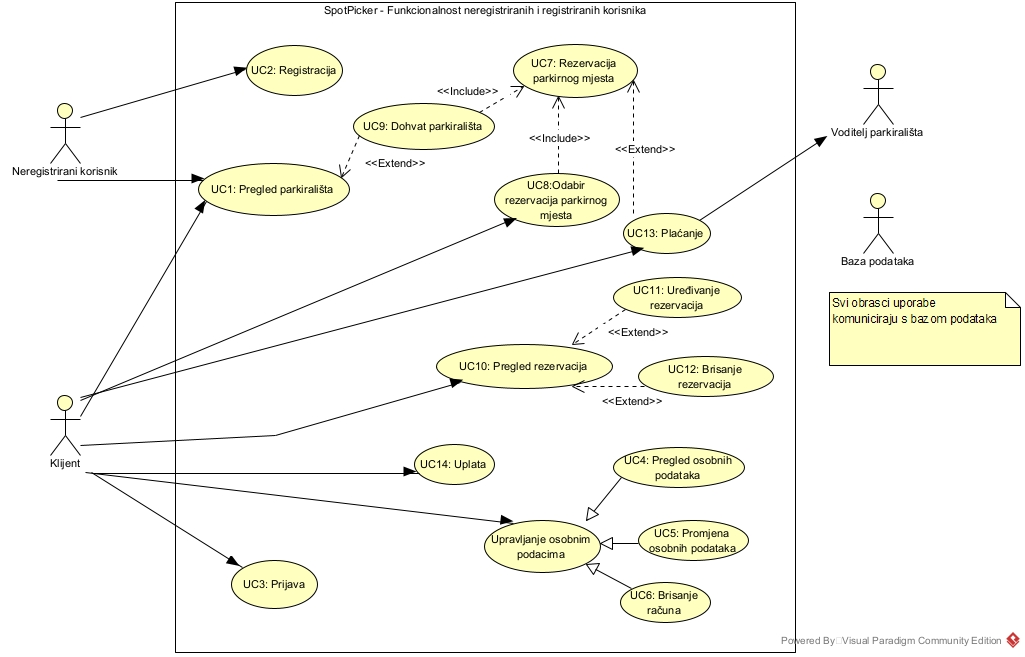
\includegraphics[width=\textwidth]{slike/UCD1.PNG} 
						\caption{Dijagram obrasca uporabe, funkcionalnost neregistriranih i registriranih korisnika}
						\label{fig:promjene6} 
					\end{figure}
					
					\begin{figure}[H]
						\centering
						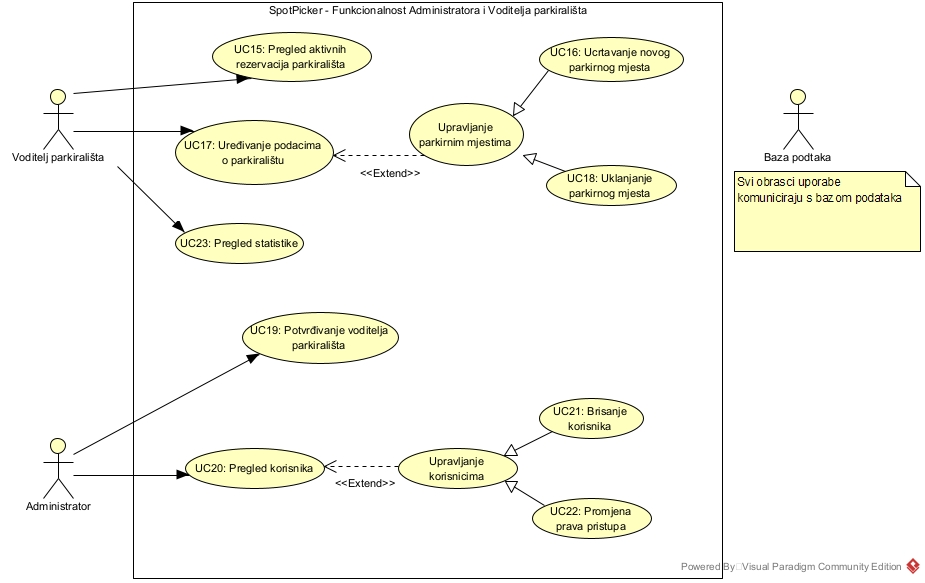
\includegraphics[width=\textwidth]{slike/UCD2.PNG} 
						\caption{Dijagram obrasca uporabe, funkcionalnost administratora i voditelja parkirališta}
						\label{fig:promjene7} 
					\end{figure}
				\eject		
				
			\subsection{Sekvencijski dijagrami}
			
				\textbf {Obrazac uporabe UC1 - Pregled parkirališta}
				
				\vspace{1cm}
				
				 Korisnik šalje zahtjev za pregledom parkirališta kako bi mogao odabrati parkirališno mjesto. Poslužitelj šalje zahtjev prema bazi podataka i dohvaća iz nje parkirališta. Ako je korisnik neprijavljen tada mu poslužitelj samo prikazuje parkirališta. Ako je riječ o prijavljenom korisniku, odnosno klijentu tada mu poslužitelj prikazuje parkirališta s informacijom o zauzetosti. Klijent zatim odabire odredište pri čemu poslužitelj šalje zahtjev prema OSRM (Open Source Routing Machine) za dohvat rute. OSRM vraća rutu poslužitelju koji ju iscrtava klijentu.  
				
				\vspace{1cm}
				
				\begin{figure}[H]
					\centering
					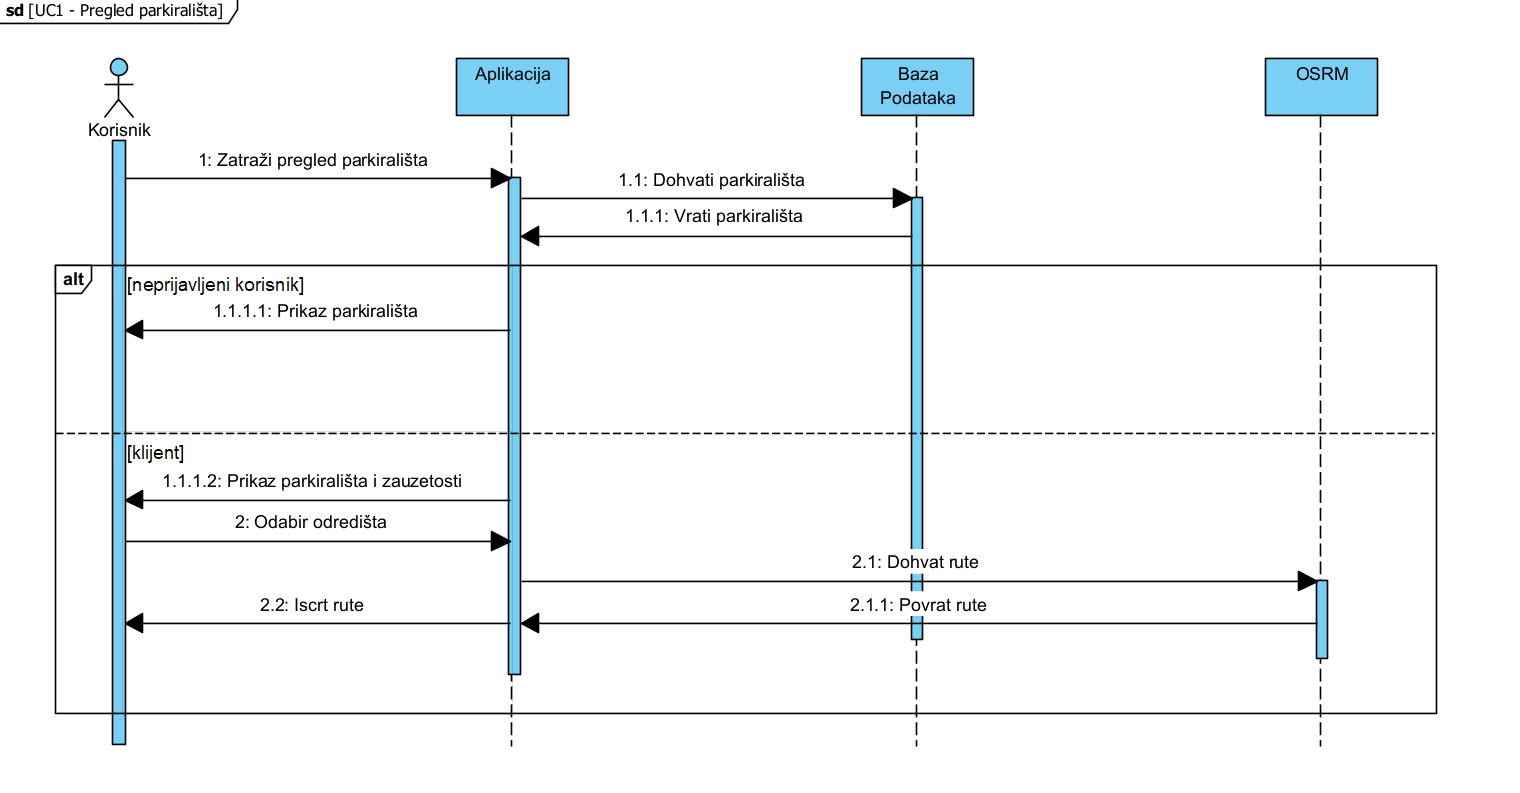
\includegraphics[width=\textwidth]{slike/SD_UC1.JPG} 
					\caption{Sekvencijski dijagram za UC1}
					\label{fig:promjene8} 
				\end{figure}
				
				\vspace{4cm}
				
				\textbf {Obrazac uporabe UC2 - Registracija}
				
				\vspace{1cm}
				
				Korisnik šalje zahtjev za registraciju sa željenom ulogom za koju se prijavljuje prema poslužitelju. Ako je željena uloga voditelj parkirališta, tada poslužitelj prima zahtjev za registraciju od korisnika i šalje prema administratoru zahtjev za potvrdu voditelja. Ako administrator potvrdi korisnika, potvrda se šalje poslužitelju. Ako je željena uloga klijent samo se šalje zahtjev za registraciju prema poslužitelju te nema potvrde administratora.
				Neovisno o ulozi koju je korisnik izabrao proces registracije se nastavlja. Poslužitelj šalje zahtjev prema bazi podataka za spremanjem korisnika. Baza podataka sprema korisnika i šalje nazad prema poslužitelju potvrdu spremanja. Konačno, poslužitelj šalje email potvrdu korisniku čime proces registracije završava.
				
				\vspace{1cm}
				
				
				\begin{figure}[H]
					\centering
					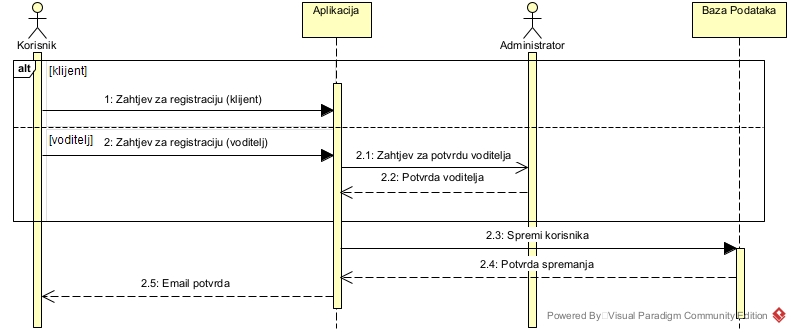
\includegraphics[width=\textwidth]{slike/SD_UC2.JPG} 
					\caption{Sekvencijski dijagram za UC2}
					\label{fig:promjene9} 
				\end{figure}
				
				\vspace{4cm}
				
				\textbf {Obrazac uporabe UC7 - Rezervacija parkirališnog mjesta}
				
				\vspace{1cm}
				
				Klijent može rezervirati parkirališna mjesta na dva načina. Prvi način je odabir po mjestu, gdje korisnik označuje željena parkirališna mjesta te šalje zahtjev prema poslužitelju. Poslužitelj zatim šalje zahtjev prema bazi podataka za dohvat dostupnih termina. Baza podataka vraća dostupne termine poslužitelju nakon čega ih poslužitelj prikazuje klijentu. Drugi način je odabir po terminu, gdje korisnik odabire željeni termin i šalje zahtjev prema poslužitelju. Poslužitelj šalje zahtjev za dohvat dostupnih mjesta prema bazi podataka. Baza podataka vraća dostupna mjesta poslužitelju koji ih prikazuje klijentu. Nakon odabira načina rezervacije klijent šalje zahtjev za definiranje rezervacije prema poslužitelju. Poslužitelj šalje zahtjev za spremanjem rezervacije prema bazi podataka te baza podataka vraća potvrdu rezervacije. Poslužitelj potvrdu rezervacije prosljeđuje nazad prema klijentu čime rezervacija parkirališnog mjesta završava.
				  
				\vspace{1cm}
				
				\begin{figure}[H]
					\centering
					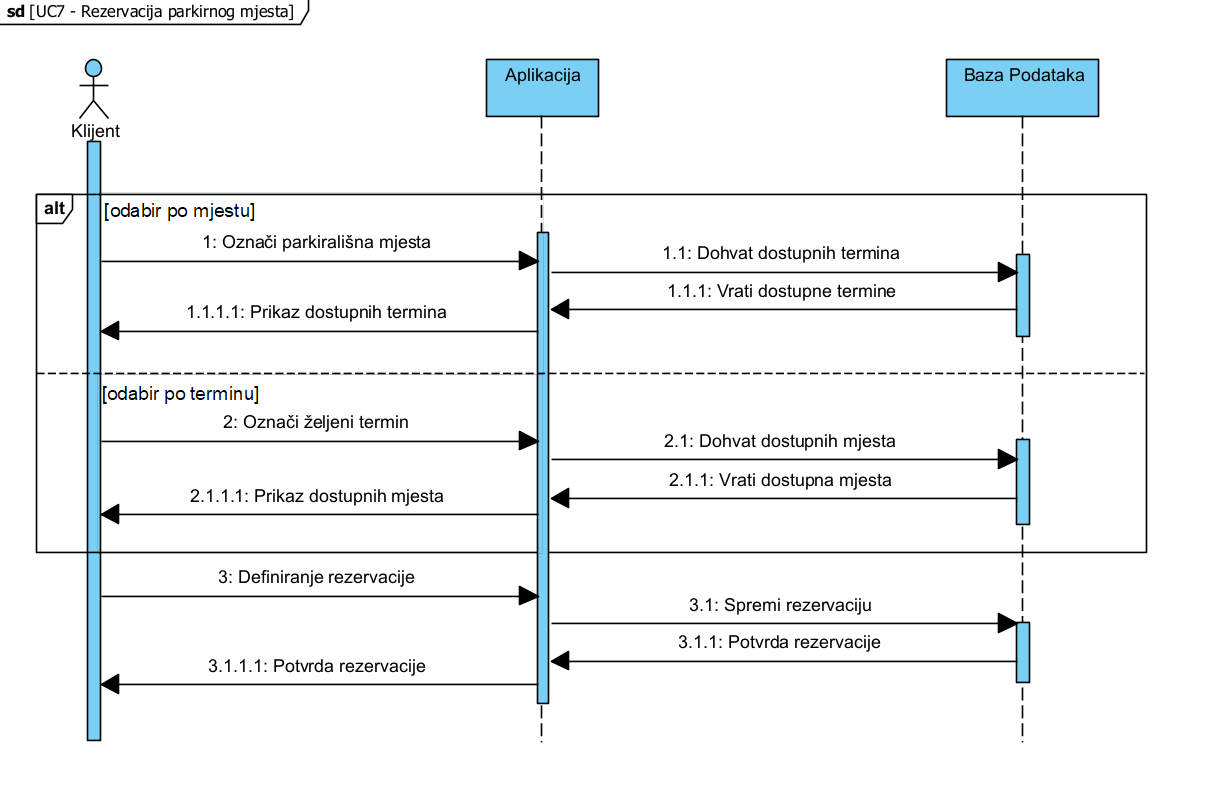
\includegraphics[width=\textwidth]{slike/SD_UC7.JPG} 
					\caption{Sekvencijski dijagram za UC7}
					\label{fig:promjene10} 
				\end{figure}
				
				\vspace{1cm}
			
				\textbf {Obrazac uporabe UC17 - Uređivanje podataka o parkiralištu}
				
				\vspace{1cm}
				
				Vlasnik šalje zahtjev za pregledom parkirališta. Poslužitelj šalje zahtjev za dohvat parkirališta prema bazi podataka. Baza podataka vraća parkirališta poslužitelju koji ih prikazuje voditelju. Voditelj traži pregled statistike zauzetosti parkirališta i parkirališnih mjesta kroz vrijeme. Poslužitelj šalje zahtjev za dohvaćanje statistike prema bazi podataka. Baza podataka vraća povijesne informacije o zauzetosti parkirališta poslužitelju. Poslužitelj na temelju dobivenih povijesnih informacija generira statistiku u obliku grafa. Dobiveni graf statistike prikazuje se vlasniku. Vlasnik šalje zahtjev za promjenu podataka poslužitelju te mu poslužitelj vraća dozvolu za pristup. Vlasnik mijenja podatke i šalje promjene poslužitelju koji promjene prosljeđuje bazi podataka. Baza podataka potvrđuje promjene i vraća potvrdu poslužitelju koji prikazuje promjene vlasniku.
				
				\vspace{1cm}
				
				\begin{figure}[H]
					\centering
					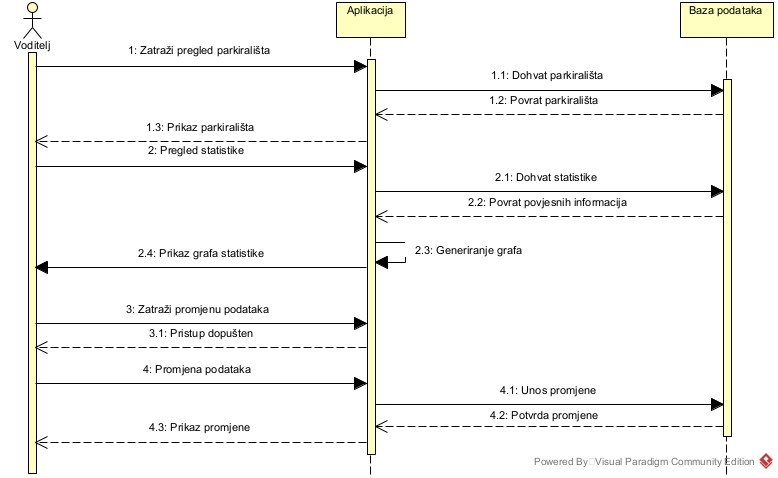
\includegraphics[width=\textwidth]{slike/SD_UC17.JPG} 
					\caption{Sekvencijski dijagram za UC17}
					\label{fig:promjene11} 
				\end{figure}

				\eject
	
		\section{Ostali zahtjevi}
		
			\textbf{\textit{dio 1. revizije}}\\
		 
			 \textit{Nefunkcionalni zahtjevi i zahtjevi domene primjene dopunjuju funkcionalne zahtjeve. Oni opisuju \textbf{kako se sustav treba ponašati} i koja \textbf{ograničenja} treba poštivati (performanse, korisničko iskustvo, pouzdanost, standardi kvalitete, sigurnost...). Primjeri takvih zahtjeva u Vašem projektu mogu biti: podržani jezici korisničkog sučelja, vrijeme odziva, najveći mogući podržani broj korisnika, podržane web/mobilne platforme, razina zaštite (protokoli komunikacije, kriptiranje...)... Svaki takav zahtjev potrebno je navesti u jednoj ili dvije rečenice.}

			 \begin{packed_enum}

				\item Koristiti OSRM za dohvat rute na mapi
				\item Koristiti Overpass API za dohvat početne informacije o parkirališnim mjestima
				\item Sustav mora biti implementiran kao web aplikacija koristeći isključivo objektno-orijentirane jezike
				\item Statistika parkirališta se prikazuje u obliku grafa
				
			 \end{packed_enum}
			 
			 

